
%(BEGIN_QUESTION)
% Copyright 2012, Tony R. Kuphaldt, released under the Creative Commons Attribution License (v 1.0)
% This means you may do almost anything with this work of mine, so long as you give me proper credit

This pictorial diagram shows the wiring connections for a simple pressure control loop, where a loop-powered 4-20 mA pressure transmitter sends a signal to a Honeywell controller, which in turn sends another 4-20 mA signal to a control valve:

$$\includegraphics[width=15.5cm]{i00974x01.eps}$$

\begin{itemize}
\item{} Sketch all directions of current, using conventional flow notation.
\vskip 10pt
\item{} Identify which electrical devices in this system act as {\it sources} and which act as {\it loads}.
\vskip 10pt
\item{} If an operator informs you that the pressure indicated by the Honeywell controller is below range (``pegged'' full downscale, reading $-25$\%), what types and locations of electrical faults might you suspect?  Are there any non-electrical faults which might also cause this to happen?
\vskip 10pt
\item{} If an operator informs you that the control valve remains fully shut no matter the output value of the controller (even in ``manual'' mode), what types and locations of electrical faults might you suspect?  Are there any non-electrical faults which might also cause this to happen?
\vskip 10pt
\item{} Suppose that a short-circuit developed between the transmitter wires in the four-conductor cable.  Explain what effect this would have on the operation of the system, as well as how you could determine that this fault was in the cable (and not in the transmitter) with your only piece of test equipment being a voltmeter.
\end{itemize}

\vskip 20pt \vbox{\hrule \hbox{\strut \vrule{} {\bf Suggestions for Socratic discussion} \vrule} \hrule}

\begin{itemize}
\item{} Review the problem-solving tips listed in Question 0 and apply them to this problem.
\end{itemize}


\underbar{file i00974}
%(END_QUESTION)





%(BEGIN_ANSWER)

$$\includegraphics[width=15.5cm]{i00974x02.eps}$$

Even though the loop-powered transmitter does exert control over the amount of current sent to the controller's input, the transmitter acts as a {\it load} rather than a {\it source}.  In other words, it functions as a {\it current regulator} while relying on the 24 VDC power supply to be the source of motive power in the circuit.
 
\vskip 10pt

A full-downscale ($-25$\%) reading at the controller suggests an {\it open} fault in the transmitter wiring somewhere, because this correlates with a zero current signal.  The fault must be electrical in nature, as no other kind of problem will cause the current in the 4-20 mA loop circuit to simply cease.

\vskip 10pt

An unresponsive control valve suggests a lack of air pressure reaching its diaphragm.  This may be caused by any kind of electrical fault in the output circuit (open or short) preventing current from reaching the I/P transducer.  It might also be the consequence of an air supply failure, or perhaps a mechanical failure inside the I/P.

\vskip 10pt

A short-circuit fault in the transmitter wiring will cause full current ($>$ 20 mA) to be sent to the controller, making it ``peg'' full upscale.  Normally, an ammeter would be a helpful tool to isolate the location of this fault, but here we only have access to a voltmeter.  In order to locate shorted faults using a voltmeter, we must break the circuit and then measure voltage ``upstream'' (toward the source) to see whether or not the shorted fault is ``downstream'' (toward the load).



%(END_ANSWER)





%(BEGIN_NOTES)







\vskip 20pt \vbox{\hrule \hbox{\strut \vrule{} {\bf Virtual Troubleshooting} \vrule} \hrule}

This question is a good candidate for a ``Virtual Troubleshooting'' exercise.  Presenting the diagram to students, you first imagine in your own mind a particular fault in the system.  Then, you present one or more symptoms of that fault (something noticeable by an operator or other user of the system).  Students then propose various diagnostic tests to perform on this system to identify the nature and location of the fault, as though they were technicians trying to troubleshoot the problem.  Your job is to tell them what the result(s) would be for each of the proposed diagnostic tests, documenting those results where all the students can see.

During and after the exercise, it is good to ask students follow-up questions such as:

\begin{itemize}
\item{} What does the result of the last diagnostic test tell you about the fault?
\item{} Suppose the results of the last diagnostic test were different.  What then would that result tell you about the fault?
\item{} Is the last diagnostic test the best one we could do?
\item{} What would be the ideal order of tests, to diagnose the problem in as few steps as possible?
\end{itemize}

%INDEX% Pictorial circuit review (4-20 mA loop)
%INDEX% Troubleshooting review: electric circuits

%(END_NOTES)


